\section{Introduction and Background}
% \section*{Introduction and Background}
% \addcontentsline{toc}{section}{Introduction and Background}
% Remove header text
\markboth{}{}
    An operating system is a computing layer that separates the hardware of the
        computer from the programs that run on it.
    It provides the \textit{environment} for other programs to do useful work
        \cite[p. 4]{textbook}.
    The fundamental tasks of an operating system include allocating resources
        (such as memory and CPU time), handling the control of input/output
        (I/O) devices, and ensuring proper usage of the computer and preventing
        errors \cite[pp. 3-5]{textbook}.

    The most important part of an operating system is the \textit{kernel}. It is
        the first program loaded into memory on startup and is the one program
        that is always running on the computer \cite[pp. 6-7, 22]{textbook}.
    Along with the kernel, operating systems also include
        \textit{middleware frameworks} that ease application development, and
        \textit{system programs} that help the system run but are not part of
        the ever-running kernel.
    All of this supports the execution of \textit{application programs}, which
        are the programs that provide functionality to the end user
        \cite[p. 4, 7]{textbook}.
    A diagram of system organization with the kernel is shown in
        \fig{kernel_in_os}.

    \begin{figure}[H]
        \centering
        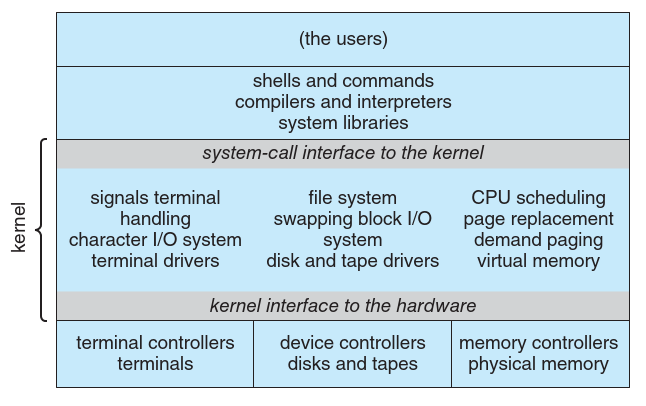
\includegraphics
            [width=0.7\textwidth]
            {images/kernel_in_os.png}
        \caption
            [Diagram of a kernel within the operating system]
            {Diagram of a kernel within the operating system \cite[p. 82]{textbook}.}
        \label{fig:kernel_in_os}
    \end{figure}

    In industrial and commercial computing applications, the choice of an
        operating system is crucial.
    It affects the performance, security, and maintainability of the system.
    As an example, consider the secure boot of an embedded system.
    Secure boot, an important security technique to ensure that the kernel code
        has not been modified, is often neglected in embedded systems.
    The absence of secure boot allows the system to boot faster with less memory
        and energy consumption---at the cost of leaving the boot process and
        internal software vulnerable.
    However, it was discovered that the introduction of secure boot software
        caused boot-up time to increase by only 4\%, whereas a hardware
        implementation of secure boot caused a 36\% increase
        \cite[pp. 11-12]{ingelhag}.
    Clearly, the operating system has a significant impact on the overall
        quality of the system.

    Two important classes of operating systems/kernels will be discussed
        here: the Linux operating system and real-time operating systems (RTOSs).
    The Linux kernel is a free and open source implementation of an operating
        system kernel.
    It is used ubiquitously not only for desktop computers, but also for servers
        and embedded devices with a broad range of commercial and
        industrial applications \cite{whatislinux}.
    The Linux kernel is a tried-and-tested system with high flexibility and
        extendability.
    RTOSs are more vague, being defined not by a specific implementation, but by
        the ability to manage systems with complex time and resource
        constraints \cite{rtos-overview}.
    RTOSs need to be able to meet strict deadlines associated with external
        events using limited resources.
    In short, ``a real-time system is one whose correctness involves both the
        logical correctness of the outputs and their timeliness''
        \cite{laplante}.

    The objective of this report is to provide a thorough comparison of the
        Linux operating system/kernel with RTOS/real-time kernels to aid in the
        decision of which operating system to use.
